\documentclass[titlepage, 10pt]{article}
\usepackage{amsmath}
\usepackage{fancyhdr}
\usepackage{geometry}
\usepackage{import}
\usepackage{titlepic}
\usepackage{graphicx}
\usepackage{lastpage}
\usepackage{float}
\usepackage{url}
\usepackage[absolute,overlay]{textpos}
\usepackage[numbib]{tocbibind}
\usepackage[tableposition=top]{caption}
\usepackage[swedish]{babel}
\usepackage[table]{xcolor}

\graphicspath{{./figures/}}

\setlength{\parindent}{0em}
\setlength{\parskip}{1em}
\setlength\headheight{14pt}


\geometry{
 a4paper,
 total={170mm,257mm},
 left=30mm,
 right=40mm,
 top=30mm,
 bottom=25mm
}

\author{Nikodemus Karlsson}
\date{November 2021}
\pagestyle{fancy}
\fancyhf{}
\rhead{\emph{Matematik specialisering}}
\lhead{Programmeringsuppgift: Minsta kvadratmetoden}
\rfoot{\thepage}

%Använde babel istället (rad 14)
%\renewcommand{\tablename}{Tabell}
%\renewcommand{\figurename}{Figur}
%\renewcommand*\contentsname{Innehåll}
%\renewcommand\refname{Referenser}

\begin{document}

\title{\large{Teori och instruktioner för}\\ \Huge{\textbf{Programmeringsuppgift}} \vspace{5mm}
\\\Large{Minsta kvadratmetoden}}
\begin{figure}
  \centering
  \titlepic{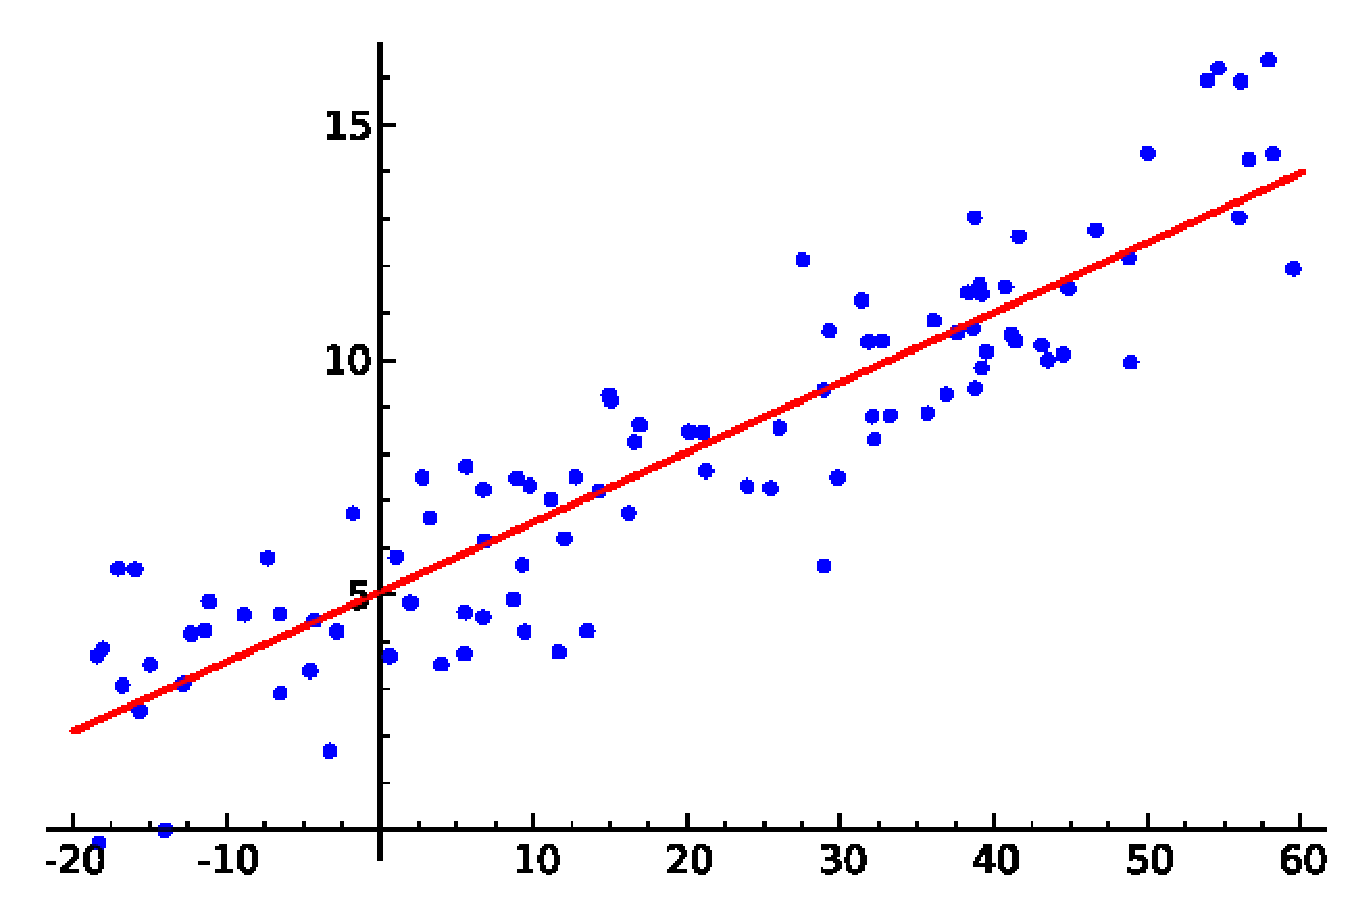
\includegraphics[scale=0.4]{640px-Linear_regression.svg.eps}}
\end{figure}
\begin{textblock*}{10cm}(15cm,28cm) % {block width} (coords) 
   \small{Typsatt med \LaTeX\\kompilerad på en Raspberry Pi}
\end{textblock*}
\author{i gymnasiekursen\\\emph{Matematik specialisering}}
\maketitle
\pagenumbering{roman}
\tableofcontents
\newpage
\pagenumbering{arabic}
\section{Inledande exempel}
Du har tidigare anpassat en rät linje till ett antal mätvärden, det används ofta
för att skapa matematiska modeller från ett begränsat antal värden. Det kan
\mbox{t ex} gälla att vi vill ta reda på hur spänningen över en resistor beror
på dess resistans givet att strömmen hålls konstant. Säg att vi har fem
resistorer som vi mäter spänningen över, och att vi får följande värden för en
och samma ström:

\begin{center}
\rowcolors{2}{gray!25}{white}
  \begin{table}[H]
    \centering
    \begin{tabular}{ |c|c|  }
    \rowcolor{gray!50}
      \hline
      Resistans, $R$ [$\Omega$] & Spänning, $U$ [V]\\
      \hline
      150 & 74.3 \\
      250 & 127\\
      450 & 230\\
      600 & 289\\
      725 & 367\\
      \hline
    \end{tabular}
    \vspace{0.5em}
    \caption{Mätvärden}
    \label{table:maetvaerden}
    \vspace{-4em}
  \end{table}
\end{center}

Detta kan plottas i ett diagram (nedanstående diagram är gjort i Google
kalkylark):

\begin{figure}[H] % H står för att figuren sätts in Här
  \centering % Centrera figuren
  \fbox{\includegraphics[scale=0.4]{cur-res.eps}}
  \caption{Plottade mätvärden}
  \label{fig:diagram}
\end{figure}

Vi ser att punkterna nästan ansluter till en rät linje med ekvationen
$y=0.497x+1.12$. Ekvationen tar kalkylarket fram åt oss med en metod som kallas
\emph{minsta kvadratmetoden}. Teorin för minsta kvadratmetoden hittar vi i den
linjära algebran. Vi ska titta lite närmare på algoritmen med vilken man får
fram ekvationen för den räta linje som ansluter bäst till ett antal punkter.
Den här uppgiften går ut på att du ska skriva ett program utifrån algoritmen
som bestämmer ekvationen för den räta linje som anpassas till ett godtyckligt
antal punkter.

\section{Minsta kvadratmetoden}
\subsection{Teckning av ekvationerna}

Om vi vill teckna förutsättningarna för en rät linje utifrån värdena i Tabell
\ref{table:maetvaerden}
så erhålls följande ekvationssystem:

\begin{equation} \label{huvudproblem}
\left\{\begin{matrix}
74.3 & = & \beta_0  & + & \beta_1 \cdot 150 \\
127 & = & \beta_0 & + & \beta_1 \cdot 250\\
230 & = & \beta_0 & + & \beta_1 \cdot 450\\
289 & = & \beta_0 & + & \beta_1 \cdot 600\\
367 & = & \beta_0 & + & \beta_1 \cdot 725\\
\end{matrix}\right.
\end{equation}

Detta ekvationssystem (\ref{huvudproblem}) saknar lösning eftersom punkterna
inte ligger på en rät linje.
Minsta kvadratmetoden går ut på att anpassa $y$-värdena så att så att det finns
tal $\beta_0$ och $\beta_1$ som gör att alla likheter uppfylls.

\textbf{Uppgift}: Skriv om ekvationssystemet på formen $A\vec{x}=\vec{y}$.

Innan vi går in på själva räknealgoritmen för Minsta kvadratmetoden så vill
jag visuellt åskådliggöra vad som händer.
\subsection{En visuell beskrivning av Minsta kvadratmetoden}

För att demonstera en metod som någorlunda enkelt påvisar om det är lösbart
eller inte så presenterar jag ett mindre system nedan. Det består av tre
ekvationer och två obekanta, och jag skriver det på formen $A\vec{x}=\vec{y}$.

\begin{equation} \label{minisystem}
  \begin{bmatrix}
    1 & -3 \\
    3 &  1 \\
    0 &  0
  \end{bmatrix}
  \begin{bmatrix}
    x_1 \\
    x_2
  \end{bmatrix}
  =
  \begin{bmatrix}
    1 \\
    -1 \\
    3
    \end{bmatrix}
\end{equation}

De båda kolonnerna i matrisen $A$, $\vec{u}=(1, 3, 0)$ och $\vec{v}=(-3, 1, 0)$
kan ses som vektorer i ett och samma plan (två vektorer i 3D bildar alltid ett
plan) medan vektorn $\vec{y}$ är en vektor som inte ligger i detta plan. Figur
\ref{fig:ortogonalprojektion} nedan illustrerar situationen
(inspirerat av \cite[p.~379]{Linalg:1})
\emph{Om} $\vec{y}$
hade legat i samma plan som $\vec{u}$ och $\vec{v}$ skulle ekvationssystemet
(\ref{minisystem}) haft en lösning.

\begin{figure}[H] % H står för att figuren sätts in Här
  \centering % Centrera figuren
  \fbox{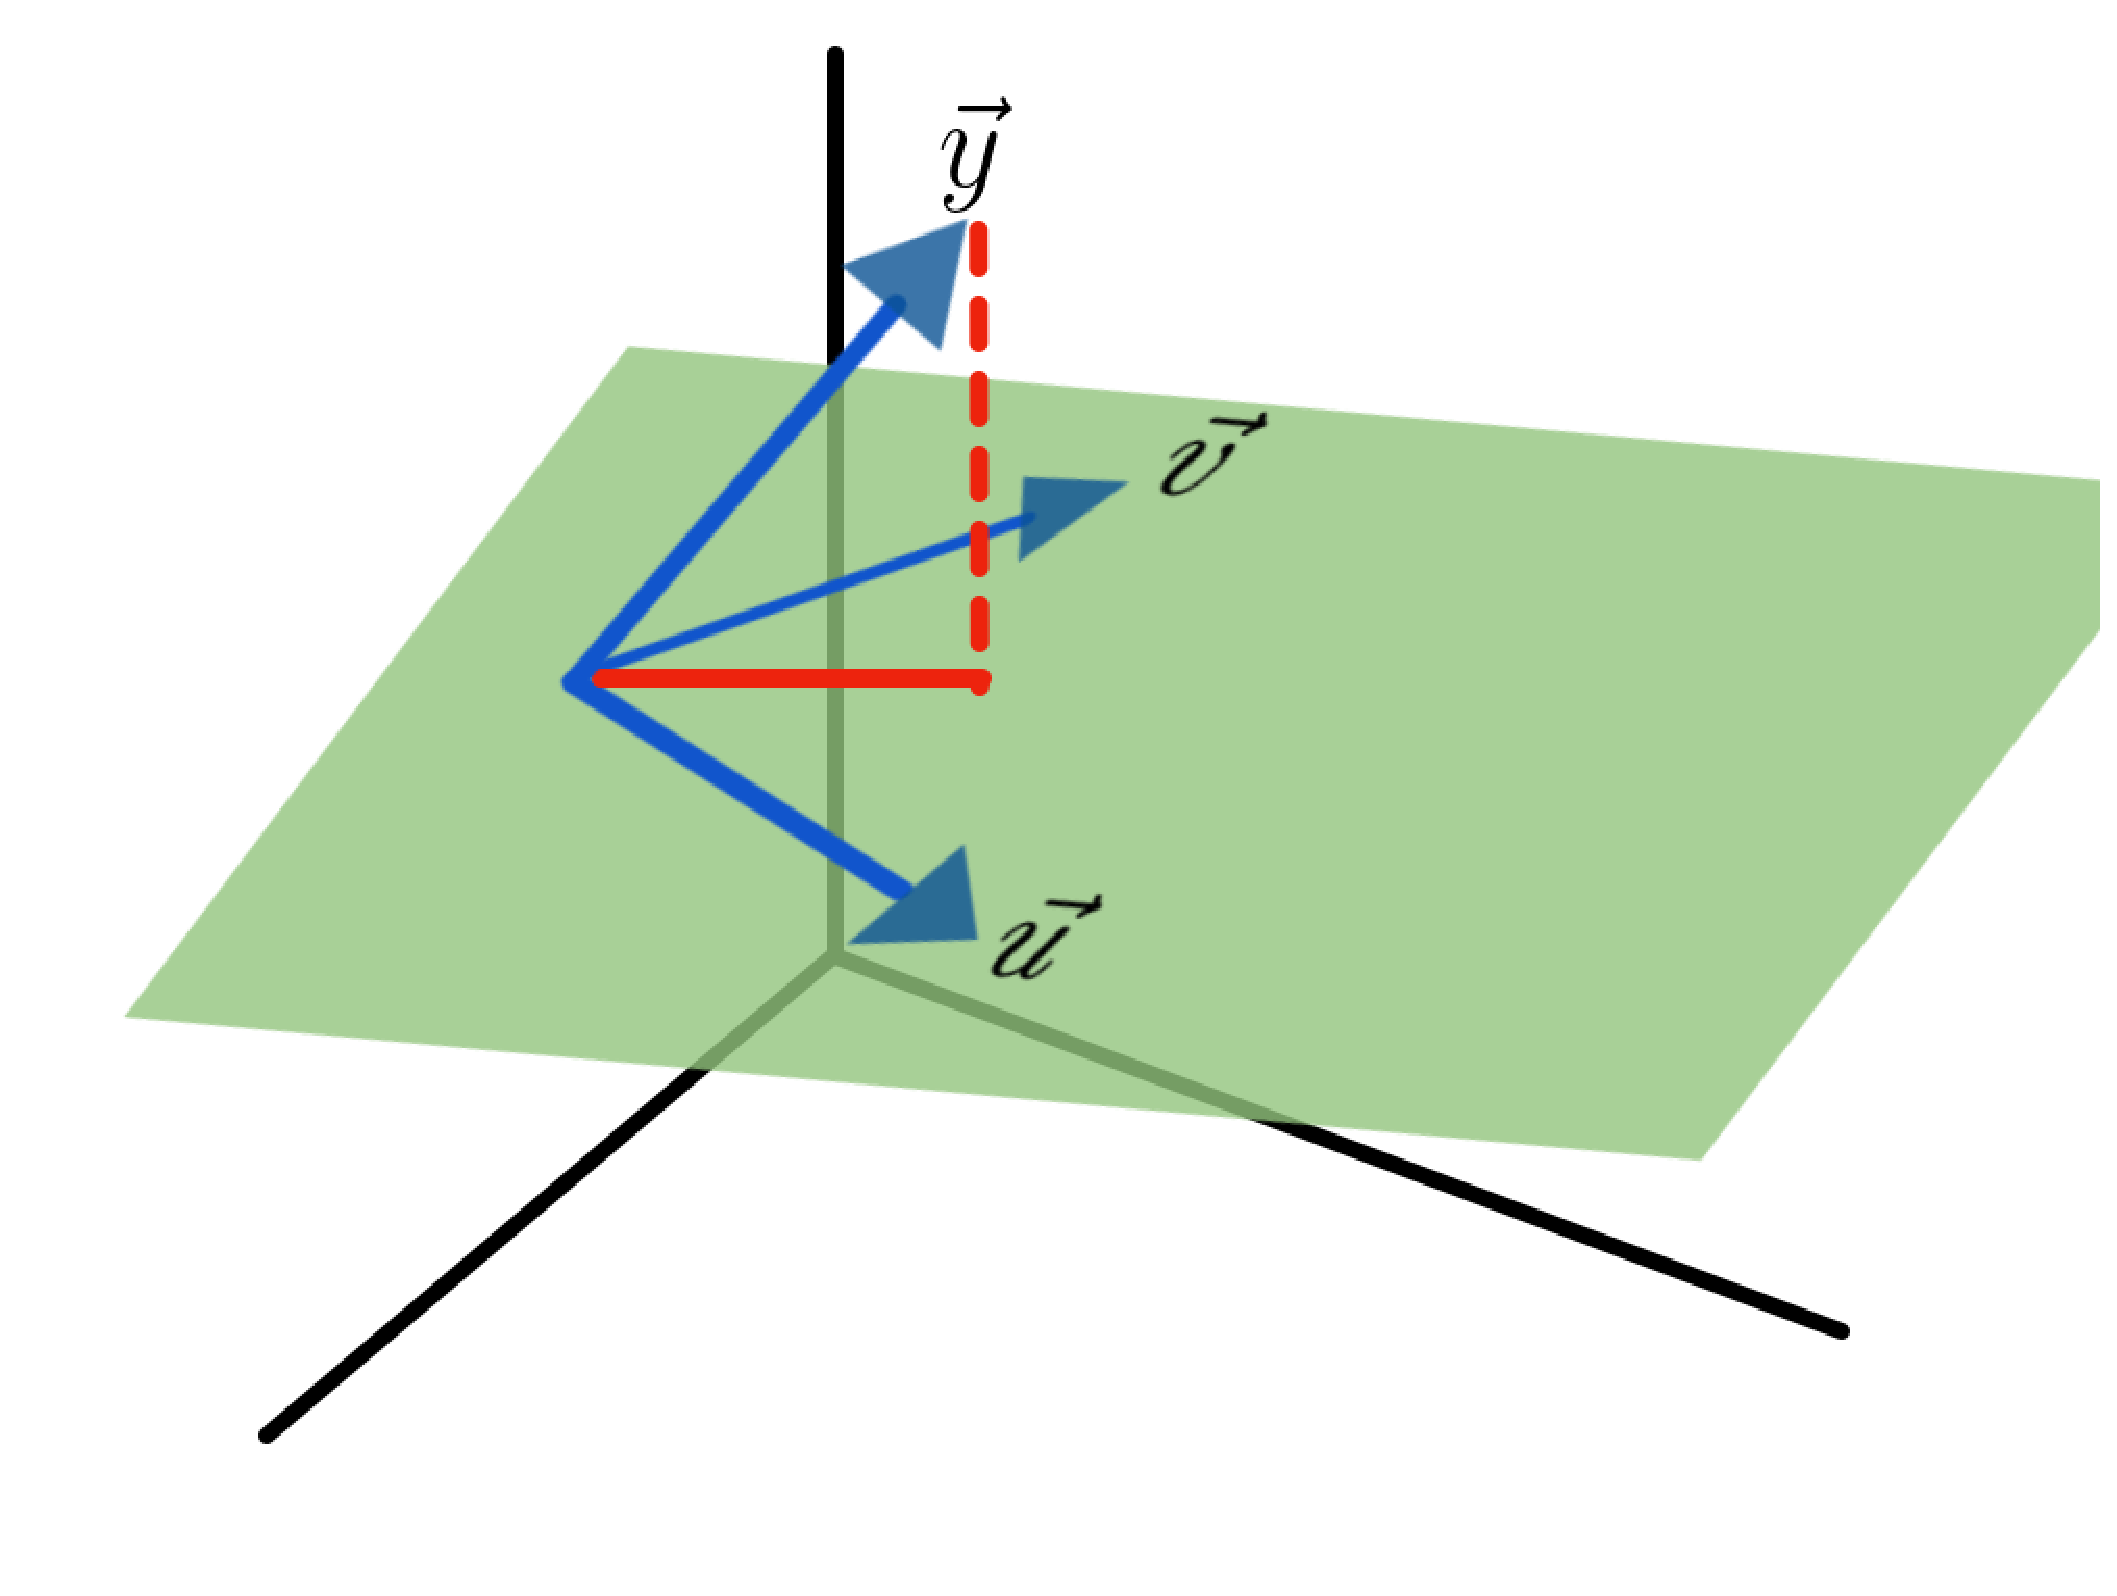
\includegraphics[scale=0.15]{projektioner.eps}}
  \caption{Vektorn $\vec{y}$ projicerad på $\vec{u}\vec{v}$-planet}
  \label{fig:ortogonalprojektion}
\end{figure}

Detta kommer sig av att lösningen måste vara en vektor som är en
linjärkombination av $\vec{u}$ och $\vec{v}$, och sådana kan inte ``bryta sig
ur'' det plan som de ingående komponenterna ligger i.

Vad gör vi då för att approximera en lösning? Jo, vi \emph{ortogonalprojicerar}
$\vec{y}$ på det aktuella planet. Det är den röda, heldragna, linjen i Figur
\ref{fig:ortogonalprojektion} som motsvarar denna ortogonalprojektion. Ju
närmare planet som $\vec{y}$ ligger från början, desto mindre kommer avvikelsen
att bli efter projektionen.

\subsection{Algoritmen för Minsta kvadratmetoden}
Nedan så presenteras den matematiska algoritmen för ortogonalprojektion.
Om du kommer att läsa en kurs i linjär algebra på högskola eller universitet
kommer den att få sin förklaring, men den ingår inte i denna gymnasiekurs.
Det finns även länk till en textmaterial med textmaterial med länkade videor i
referenserna nedan för den som redan nu är nyfiken.

För att ortogonalprojicera multipliceras från vänster med $A^T$ på båda sidor
\cite[p.~85]{MatrixAlgebraForEngineers:1}.
$A^T$ är \emph{trans\-ponatet} till $A$, vilket innebär att raderna blir
kolonner och kolonnerna blir rader. \mbox{T ex} gäller

\begin{equation}
  A =
  \begin{bmatrix}
    1 & -3 \\
    3 &  1 \\
    0 &  0
  \end{bmatrix} \Rightarrow
  A^T =
  \begin{bmatrix}
    1 & 3 & 0 \\
    -3 &  1 & 0
  \end{bmatrix}
\end{equation}

Ekvationssystemet (\ref{huvudproblem}) tecknas på matrisform som

\begin{equation}
  \begin{bmatrix}
    1 & 150 \\
    1 & 250 \\
    1 & 450 \\
    1 & 600  \\
    1 & 725
  \end{bmatrix}
  \begin{bmatrix}
    \beta_0 \\
    \beta_1
  \end{bmatrix}
  =
  \begin{bmatrix}
    74.3 \\ 127 \\ 230 \\ 289 \\ 367
  \end{bmatrix}
\end{equation}

Med metoden att multiplicera med transponatet så erhålls

\begin{equation}
  \begin{bmatrix}
    1 & 1 & 1 & 1 & 1 \\
    150 & 250 & 450 & 600 & 725
  \end{bmatrix}
  \begin{bmatrix}
    1 & 150 \\
    1 & 250 \\
    1 & 450 \\
    1 & 600  \\
    1 & 725
  \end{bmatrix}
  \begin{bmatrix}
    \beta_0 \\
    \beta_1
  \end{bmatrix}
  =
    \begin{bmatrix}
    1 & 1 & 1 & 1 & 1 \\
    150 & 250 & 450 & 600 & 725
    \end{bmatrix}
    \begin{bmatrix}
    74.3 \\ 127 \\ 230 \\ 289 \\ 367
    \end{bmatrix}
\end{equation}

Detta kan se klurigt ut, men det är enbart matrismultiplikation (som dessutom
ska göras på dator eftersom det är en programmeringsövning). Resultatet kommer
att bli

\begin{equation}
  \begin{bmatrix}
    5 & 2\,175 \\
    2\,175 & 1\,173\,100
  \end{bmatrix}
  \begin{bmatrix}
    \beta_0 \\ \beta_1
  \end{bmatrix}
  =
  \begin{bmatrix}
    1\,087.3 \\ 585\,870
  \end{bmatrix}
\end{equation}

Vi ser att det är ett system med två ekvationer och två obekanta (så kommer det
alltid att bli när en rät linje ska approximeras). Sådana system är enkla att
lösa eftersom det finns en metod med få steg att invertera den ingående
$2\times 2$-matrisen (se kap. 1 i kurskompendiet
\cite{Linalgkompendium:1}). Just det här
ekvationssystemet får lösningen $\beta_0=1.120$ och $\beta_1=0.497$. Det innebär
att vi kan approximera en linje genom punkterna med ekvationen $y=0.497x+1.12$
(där $y$ är spänningen och $x$ är resistansen i exemplet med mätvärden i Tabell
\ref{table:maetvaerden}). Det är exakt detsamma som Google kalkylark beräknade
åt oss i Figur \ref{fig:diagram}.

\section{Uppgift}
\subsection{Uppgiftsformulering}
Du ska skriva ett program i Python som implementerar Minsta kvadratmetoden
enligt ovanstående beskrivning av algoritmen.
I själva huvudprogrammet ska \texttt{x}-vektorn och \texttt{y}-vektorn anges
separat, det är dessa som kommer att motsvara kolumnerna med värden i Tabell
\ref{table:maetvaerden}.
Det ska kunna vara ett godtyckligt antal par av mätvärden i respektive vektor.
Dessa ska sedan skickas till en funktion som returnerar de eftersökta värdena på
$\beta_0$ och $\beta_1$ (som är definierade i ekvationssystem
(\ref{huvudproblem})).

\subsection{Tips}
\begin{itemize}
  \item Börja med att utföra importen av \texttt{NumPy}: \texttt{import numpy as
  np}
  \item Skapa dina vektorer \texttt{x} och \texttt{y} som \texttt{matrix},
  \mbox{t ex} \texttt{x = np.matrix([1, 2, 3])}.
  \item För att skapa en tom matris med $m$ rader och 2 kolonner kan du använda
  \texttt{A = np.empty((m, 2))} (där $m$ är antalet element i \texttt{x}-
  vektorn)
  \item För att ersätta en kolonn med en vektor \texttt{v} i matrisen \texttt{A}
  kan du utföra \texttt{A[:,1] = v}. Detta ersätter kolonnen med ordningsnummer
  1, dvs den andra kolonnen (\texttt{NumPy} är nollindexerat). Här gäller att
  vektorn \texttt{v} måste vara en radvektor med lika många element som matrisen
  \texttt{A} har rader.
  \item Matriser kan transponeras med metoden \texttt{transpose}, \mbox{t ex}
  \texttt {A.transpose()}. Det brukar vara bra att spara transponatet
  i en separat variabel, \mbox{t ex} \texttt{A\_T = A.transpose()}.
  \item En matris kan multipliceras med en annan matris eller vektor (av rätt
  dimension, förstås) med \texttt{@}-operatorn, \mbox{t ex} \texttt{AB = A@B}.
  \item En matris, \mbox{t ex} \texttt{A}, kan inverteras genom att utföra
  \texttt{np.linalg.inv(A)}. Det brukar vara bra att spara inversen i en separat
  variabel, \mbox{t ex} \texttt{A\_inv = np.linalg.inv(A)}.

\end{itemize}

\newpage
%\section{Referenser}
\bibliography{referenser} 
\bibliographystyle{ieeetr}
\end{document}
